\subsection{RQ2 --- Are the explanations correct, and does encryption change that?}
\label{sec:rq2}
\begin{itemize}[leftmargin=*, itemsep=0pt]
  \item \textbf{Quality is moderate and depends on the explainer.} Faithfulness is mostly 0.2--0.6 (Table~\ref{tab:costfid}). The best explainer for each detector is a fast one: TreeSHAP for XGBoost (0.60 on CIC-IDS2017, 0.46 on HIKARI), IG for the MLP (0.56 and 0.45), and the EBM's own explanations on HIKARI (0.70). Infidelity and deletion AOPC rank the explainers similarly (Spearman correlation with faithfulness 0.79 and 0.45 on CIC-IDS2017, 0.48 and 0.79 on HIKARI).
  \item \textbf{A bigger budget helps only up to a point.} KernelSHAP with 100 samples is useless (faithfulness about 0), while 500 samples are as good as 2{,}048. More LIME samples or IG steps add little.
  \item \textbf{DeepSHAP is unreliable} for our MLP (faithfulness 0.09--0.30, and unstable on HIKARI).
\end{itemize}

\textbf{Does encryption make explanations worse? Not on CIC-IDS2017.} Hypothesis H2 expected lower quality on $T_3$. Table~\ref{tab:tier} shows the opposite on CIC-IDS2017: faithfulness is significantly \emph{higher} on $T_3$ for 7 of 8 pairs, for example KernelSHAP on XGBoost rises from 0.29 to 0.49. The reason is that with all features, half of XGBoost's explanation weight sits on ports and TCP flags, which are known recording artefacts of this dataset~\cite{engelen2021}. On $T_3$ the weight moves to packet-size statistics, which describe the traffic itself and are easier to explain. On HIKARI the result is mixed: 3 pairs get worse, 1 gets better and 4 do not change. Features do become more correlated on $T_3$, as expected (mean $|\rho_s|$ 0.36 $\rightarrow$ 0.43 on CIC-IDS2017).

\begin{table}[!htbp]
\centering
\caption{Faithfulness with all features ($T_1$) and with the encrypted-traffic view ($T_3$) on the same flows. $p$ = paired Wilcoxon test, Holm-corrected.}
\label{tab:tier}
\scriptsize
\setlength{\tabcolsep}{2.5pt}
\begin{minipage}[t]{0.495\textwidth}
\centering
\begin{tabular}{llrrrr}
\toprule
\multicolumn{6}{c}{\textbf{CIC-IDS2017}} \\
\midrule
\textbf{Model} & \textbf{Explainer} & \textbf{$T_1$} & \textbf{$T_3$} & \textbf{$\Delta$} & \textbf{$p$} \\
\midrule
MLP & DeepSHAP & 0.23 & 0.30 & 0.07 & 7e-04 \\
MLP & IG-32 & 0.47 & 0.56 & 0.09 & 3e-07 \\
MLP & KernelSHAP-500 & 0.29 & 0.32 & 0.03 & 0.22 \\
MLP & LIME-1000 & 0.22 & 0.28 & 0.06 & 4e-03 \\
XGB & KernelSHAP-500 & 0.29 & 0.49 & 0.20 & 2e-14 \\
XGB & LIME-1000 & 0.23 & 0.30 & 0.07 & 2e-04 \\
XGB & TreeSHAP-interv & 0.35 & 0.52 & 0.17 & 1e-14 \\
XGB & TreeSHAP-path & 0.52 & 0.60 & 0.08 & 3e-05 \\
\bottomrule
\end{tabular}
\end{minipage}
\hfill
\begin{minipage}[t]{0.495\textwidth}
\centering
\begin{tabular}{llrrrr}
\toprule
\multicolumn{6}{c}{\textbf{HIKARI-2021}} \\
\midrule
\textbf{Model} & \textbf{Explainer} & \textbf{$T_1$} & \textbf{$T_3$} & \textbf{$\Delta$} & \textbf{$p$} \\
\midrule
MLP & DeepSHAP & 0.10 & 0.09 & -0.02 & 0.69 \\
MLP & IG-32 & 0.49 & 0.45 & -0.04 & 0.69 \\
MLP & KernelSHAP-500 & 0.14 & 0.02 & -0.12 & 9e-13 \\
MLP & LIME-1000 & 0.27 & 0.25 & -0.02 & 0.69 \\
XGB & KernelSHAP-500 & 0.28 & 0.23 & -0.05 & 0.02 \\
XGB & LIME-1000 & 0.16 & 0.21 & 0.05 & 4e-03 \\
XGB & TreeSHAP-interv & 0.35 & 0.27 & -0.08 & 1e-07 \\
XGB & TreeSHAP-path & 0.49 & 0.46 & -0.03 & 0.69 \\
\bottomrule
\end{tabular}
\end{minipage}
\end{table}


\textbf{Explainers disagree.} Two explainers share on average only about 2 of their top-5 features (Jaccard@5 0.19--0.31 for the tree models and the MLP; Fig.~\ref{fig:agreement}). Only two methods that estimate the same quantity agree well (KernelSHAP-2048 and interventional TreeSHAP: 0.71). The explanation an analyst sees therefore depends on the chosen explainer, so its quality has to be measured, not assumed.

\begin{figure}[!htbp]
\centering
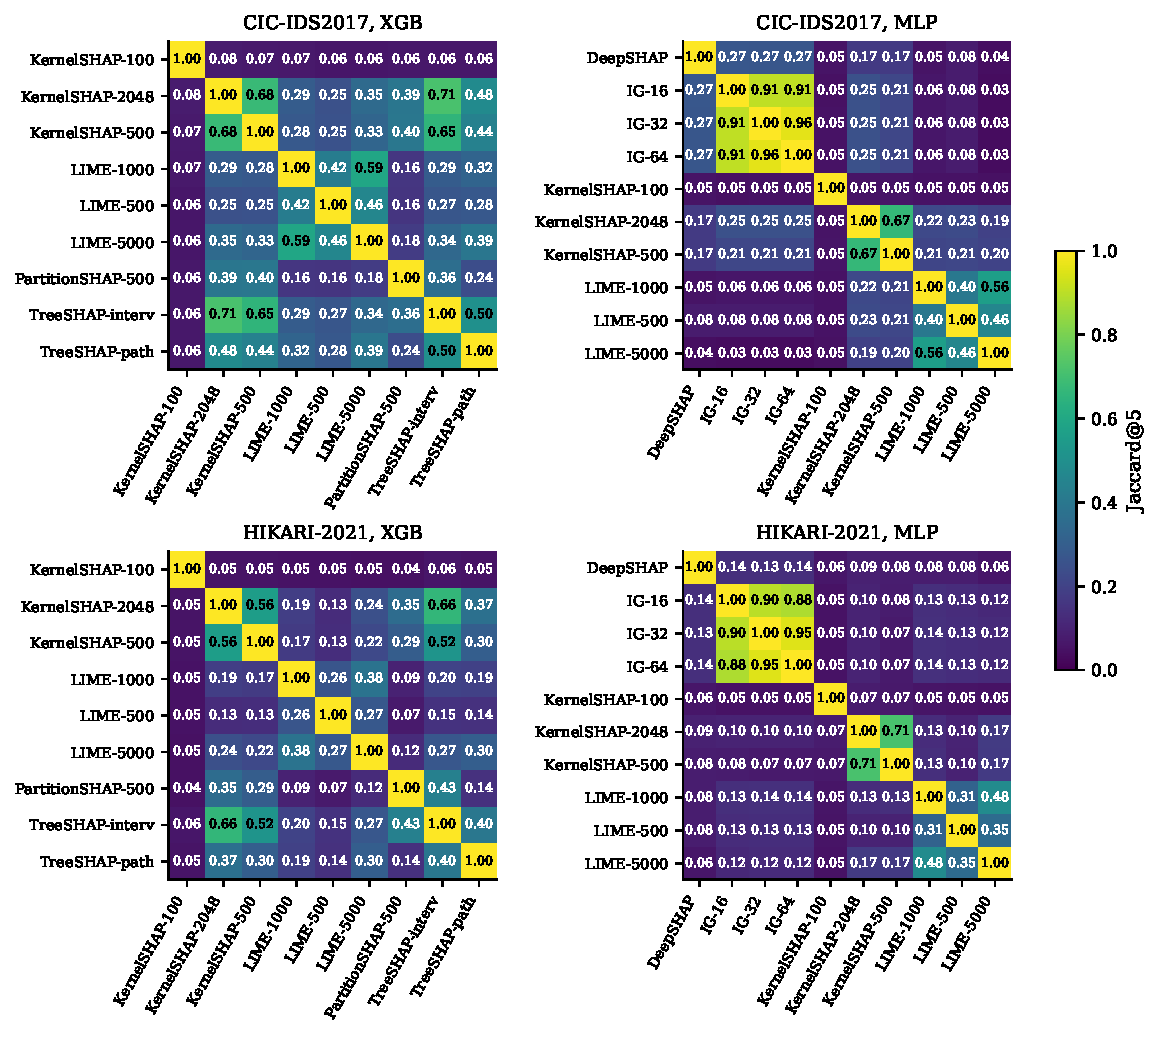
\includegraphics[width=0.72\textwidth]{../figures/fig_agreement.pdf}
\caption{Top-5 agreement (Jaccard@5) between explainers on the same flows ($T_3$).}
\label{fig:agreement}
\end{figure}
